\documentclass[a4paper,10pt,hidelinks]{scrartcl}

% packages
\usepackage[english]{babel}
\usepackage{graphicx}
\usepackage{hyperref}
\usepackage{url}
\usepackage{fontspec}
    \setmainfont{Arial}
    \setsansfont{Arial}
    \setmonofont{Fira Code}
\usepackage{fancyhdr}
\usepackage[paper=a4paper,left=20mm,right=20mm,top=40mm,bottom=25mm,headheight=40mm]{geometry}
\usepackage{tabto}
\usepackage{sectsty}
\usepackage{afterpage}
\usepackage{listings}
\usepackage{blindtext}
\usepackage{float}
\usepackage{wrapfig}

\hypersetup{
    colorlinks=true,
    linkcolor=black,
    filecolor=blue,      
    urlcolor=blue,
}

% global options
\renewcommand{\baselinestretch}{1.25}

\lstset{basicstyle=\small\ttfamily,captionpos=b,xleftmargin=0.25in,xrightmargin=0.25in}

% header/footer
\pagestyle{fancy}
\renewcommand{\headrulewidth}{0pt}
\renewcommand{\footrulewidth}{0pt}
\rhead{
\includegraphics[width=40mm]{pics/header-2.png}}
\rfoot{
\includegraphics[width=40mm]{pics/footer.png}}
\fancypagestyle{firstpage}{
    \rhead{
\includegraphics[width=40mm]{pics/header-1.png}}
}
\cfoot{}

\newcommand{\imgref}[1]{{figure \ref{#1}}}

\begin{document}

\section*{\fontsize{18}{20}\selectfont Object detection in fine-art photography}
\thispagestyle{firstpage}

\textbf{Themenbereiche:} \tabto{4cm} Artificial Intelligence, Visual Computing

\noindent
\textbf{Studierender:} \tabto{4cm} Fabian Meyer

\noindent
\textbf{Betreuungsperson:} \tabto{4cm} Dr. Simone Lionetti

\noindent
\textbf{Experte:} \tabto{4cm} Roman Bachmann, Swisscom

\noindent
\textbf{Keywords:} \tabto{4cm} Object detection, Machine learning, Computer vision, Photography

\section{\fontsize{14}{16}\selectfont Task description}

Object detection is an important computer vision and machine learning task that consists in the localisation and classification of items within digital images. The business and industry applications of this technology are growing in number and relevance, especially because of the tremendous progress, largely driven by deep learning, that has been made in recent years.

The aim of this work is to develop a web-application that is built around an object-detection model. This web-application takes in pictures, looks for objects in it and returns a "tidied up" image with the objects found in it. 

This "tidied up" image is inspired by "Kunst aufräumen", a series of fine-art photographies by Swiss artist Urs Wehrli, that consists of two images, a "messy" one and a "tidy" one.

In a further step, an existing model was refined by retraining it on a dataset with three images from "Kunst aufräumen" and the performance of the two models where examined.

\section{\fontsize{14}{16}\selectfont Results}

A dataset consisting of 42 images from four different artists has been gathered. The frameworks TensorFlow, Detectron2 and MMDetection have been tried out on Google Colab on this dataset with each an implementation of an instance segmentation model. MMDetection has been chosen as it has a very high-level API. Mask R-CNN has been chosen as the model to use further, as it had the better performance compared to CenterNet. The model chosen has a ResNet-101 backbone and contains a feature-pyramid-network. With the MMDetection framework and this model, a web-application has been developed. The web-application has been deployed on the EnterpriseLab. It can be accessed at: \url{http://bdaf20-iameyer.enterpriselab.ch}. In a further step, the existing Mask R-CNN model has been taken and retrained on Google Colab with fine-art photography data from the series "Kunst aufräumen". The performance of the out-of-the-box model and the retrained model has been compared.

In sum the performance of the pretrained on COCO-dataset Mask R-CNN model depends on the following criteria: The class of objects depicten in the image (included in COCO-dataset or not), the size of objects in the image and the degree to which an object is visible and is shown in a natural style.

When applied to images of fine-art photography we can observe that performance of object-detection models is variable to some extend because different photographers use different styles to depict their objects in their images. For example when using an image with a lot of smaller objects (like Andreas Gursky does), performance is rather poor compared to an image with fewer and bigger objects. %TODO retraining

\section{\fontsize{14}{16}\selectfont Solution}

\begin{wrapfigure}{r}{0.333\textwidth}
	\center{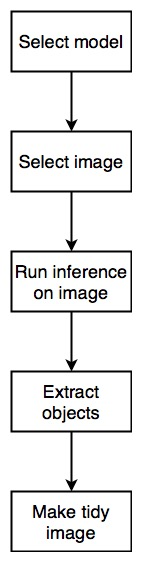
\includegraphics[width=75pt]
	{pics/control-flow.jpg}}
	\caption{\label{fig:control-flow} Control-flow diagram}
\end{wrapfigure}

The web application analyses images which can either be selected from a predefined list or uploaded by the user or fetched via a url. Then inference is run on the chosen image. The chosen model detects potential objects in the image and returns them as a data structure, containing masks, bounding-boxes, name of class and confidence score. \newline The program reads these four results and cuts out all objects from the original image. The found objects will be depicted on a new image in a grid-like fashion. One can see a high-level view of the program in image: \imgref{fig:control-flow}.

Cutting out the objects is possible with the help of the bounding-box and the mask of one object alone.

As there are a lot of frameworks and libraries for deep-learning and object detection that are using Python as their main programming-language, Python has been chosen as the language to develop the full project. To transform the program into a full working web application, \href{https://dash.plotly.com}{Plotly Dash} has been chosen. Dash is using HTML-, CSS-, and JavaScript-technologies under the hood to get a Python app running on a web server.

For the framework, \href{https://github.com/open-mmlab/mmdetection/}{mmdetection} has been chosen because of its high level API and vast array of models avaiable. As mmdetection (like most frameworks) needs a GPU for training and inference, \href{https://github.com/akarazniewicz/smd}{smd} (a wrapper around mmdetection models) is used as a way to perform inference on CPU.

A sample input image from "Kunst aufräumen" and the corresponding output is shown in \imgref{fig:input-image} and \imgref{fig:output-image}.

\begin{figure}[!h]
	\center{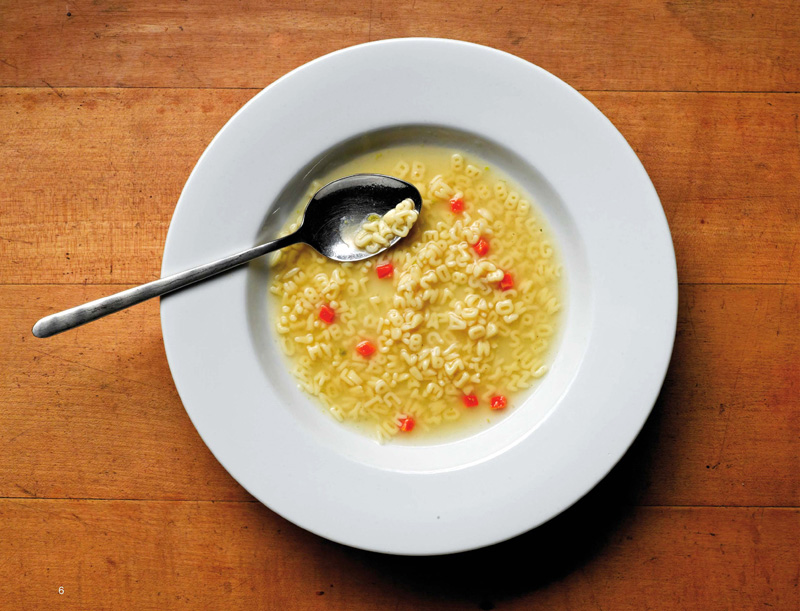
\includegraphics[width=175pt]
	{pics/input.jpg}}
	\caption{\label{fig:input-image} Sample input image}
\end{figure}

\begin{figure}[!h]
	\center{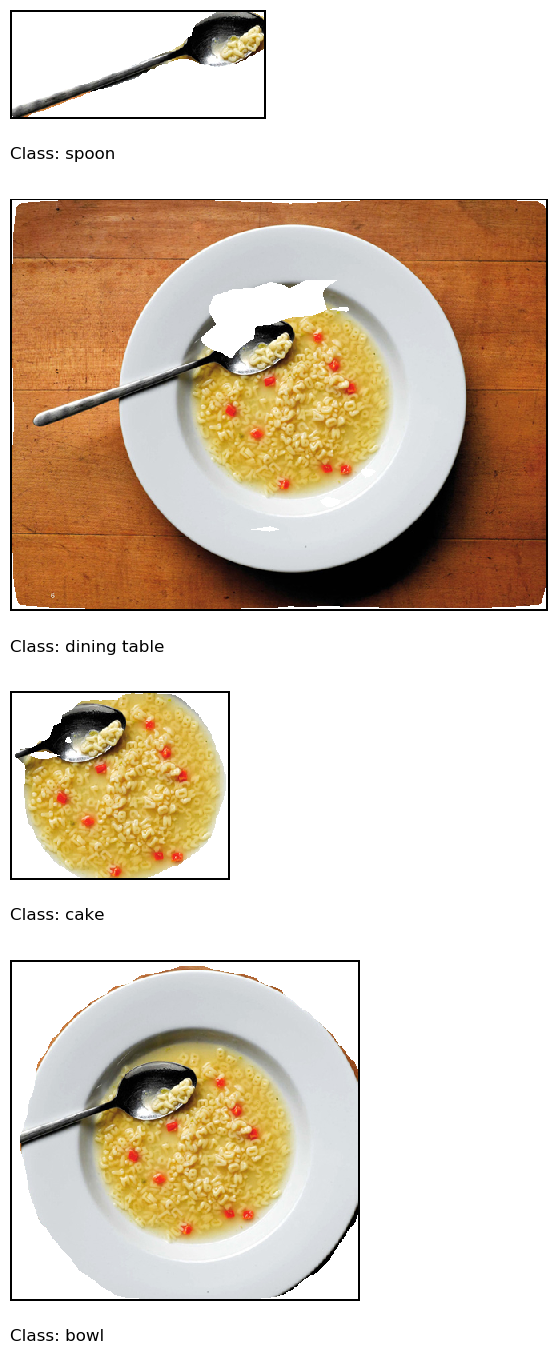
\includegraphics[width=175pt]
	{pics/output.jpg}}
	\caption{\label{fig:output-image} Sample output image}
\end{figure}

\section{\fontsize{14}{16}\selectfont Challenges}

One big challenge was, that at the time of writing, MMDetection did not support inference performed on CPU. As a consequence, a wrapper around the existing model is used to get a model running on a standard CPU, for development purpose but also for deployment on a server. As most deep-learning networks are trained with GPUs, the easiest (and also most performant) way to deploy an app would be to use a GPU environment. Using a CPU for inference results in much longer computation time. This is a big drawback, in terms of user experience.

\section{\fontsize{14}{16}\selectfont Outlook}

After the experience of using an existing model for detecting objects in fine-art photography and retraining it with sample data from artistic photography, more models could be retrained to gain a deeper understanding of the detection of objects in images from different photographers. In a future work one could for example train a model on images from one photographer and test it on images from another photographer that contains the same classes of objects in it. In technical terms it would be interesting to decrease the computation time as much as possible, either by using a GPU-powered environment for deployment or by using a more recent framework that supports sufficiently fast computation on CPU.

\end{document}
